\chapter{Results and Experiments} % Main chapter title

\label{chapter:observer_results} % Change X to a consecutive number; for referencing this chapter elsewhere, use \ref{ChapterX}

\lhead{Chapter 4. \emph{Results and Experiments}} % Change X to a consecutive number; this is for the header on each page - perhaps a shortened title

This chapter presents an experiment used to evaluate the intention recognition capacity of our system. Section~\ref{sec:observer_experiment-case_study} introduces our case study, where we decided to compare the prediction of our system with those of humans. Section~\ref{sec:observer_experiment-experiment} explains how the experiment was actually conducted. We show and discuss our results in section~\ref{sec:observer_experiment-discussion}.


\section{Case Study}
\label{sec:observer_experiment-case_study}
\subsection{Study Description}

Evaluating the capacity of the system to estimate human intentions is not easy, since intentions are not directly observable. A possible solution, as shown in~\cite{baker2014modeling}, is comparing the estimation of human intentions, performed by other humans, with the predictions of our system. In order to perform this comparison we created a user study where we showed participants several videos, asking them to estimate the likelihood of a set of intentions  for each video, and collected their results. The same tests were simulated on the system, streaming as input a sequence of observations  corresponding to the actions shown in the video (e.g. if the video shows a human approaching the table, we will stream to the system a trajectory of coordinates that leads to the table position). All of the test videos ended in a situation of ambiguity. For example, in one test we showed a human approaching a table with different objects, and stopped the video before users could see which object the human wanted to take. Some videos include more information than others, like comments by humans or situations that help to disambiguate the intention. 

We have performed an equivalence test, comparing users' intentions predictions with those of the system, following the two one-sided tests (TOST) approach. We choose as a threshold for equivalence the standard deviation $\sigma$ of the users' answers. The idea behind this choice is that, if the system's answers are closer than a standard deviation to the average human answers, its predictions are comparable to an average human answer from our user group. 

We defined our hypothesis as follow: 
\begin{itemize}
\item $H_0$: $\mu_{hi}-\mu_{si}\leq-\sigma_{hi}$ \; \text{OR} \; $\mu_{hi}-\mu_{si}\geq\sigma_{hi}$ 
\item $H_A$: $-\sigma_{hi}<\mu_{hi}-\mu_{si}<\sigma_{hi}$  
\end{itemize}
where $\mu_{hi}$ and $\mu_{si}$ are the human average and the system's answer for test $i$, $\sigma_{hi}$ is the variance of the human answers for test $i$.

We have performed tests to evaluate: a) prediction in absence of clues, b) prediction in the presence of contextual clues, c) prediction in the presence of belief state clues.

We have built a household environment with a fixed set of furniture: a \textit{Kitchen Shelf}, a \textit{Table}, a \textit{Sofa}, and a \textit{Chair}. In this environment, we have created two scenarios, composed by several tests, with two agents, \textit{Max} and \textit{Bob}, performing different actions. Each scenario contained a set of objects, and a constrained set of intentions. For the tests related to belief states, we start by showing the users a specific sequence of events, allowing them to build a mental model of the agents. A corresponding simulated sequence will be streamed to the system for this test.
We will describe in details the two scenarios and the relative tests.

\subsection{Cookie Scenario}
\begin{itemize}
\item Objects: a \textit{Cookie Box}, a \textit{Mug}, and a \textit{Bottle of Water} were placed on the \textit{Table}, close to each other. A pack of \textit{Cookies} was placed on the \textit{Kitchen Shelf}. The \textit{Cookie Box} could contain, or not, \textit{Cookies}.
\item Intentions: \textit{Eating a Cookie}, \textit{Drinking Water}, \textit{Reading the Book}.
\item Tests:
\begin{itemize}
	\item \textit{No Clues}: \textit{Max} approaches the \textit{Table}.
    \item \textit{Contextual Clues}: \textit{Max} approaches the \textit{Table} commenting on the warmth of the day.
	\item \textit{Divergent Belief No Cookies}: \textit{Max} approaches the \textit{Table}.
	\item \textit{Divergent Belief Cookies}: \textit{Bob} approaches the \textit{Table}.
\end{itemize}
\item  \textit{Divergent Belief Event}:  \textit{Max} and \textit{Bob} are chatting on the \textit{Sofa}. Max eats the last \textit{Cookie} from the \textit{Cookie Box} before closing it and leaving. While \textit{Max} is away, \textit{Bob} takes \textit{Cookies} from the \textit{Kitchen Shelf}, fills the \textit{Cookie Box} with them, and closes it, before leaving.
\end{itemize}

The \textit{Divergent Belief Event} was shown to the users (and its simulation streamed to the system) between the \textit{Contextual Clues} and the \textit{Divergent Belief No Cookiies} events. 


We have deliberately included an intention, \textit{Reading the Book}, without placing a book in the visible environment, introducing a confusing element in the scenario. This scenario can be seen in figure~\ref{fig:observer_experiments-cookie}.


 \begin{figure}[ht!]
	\centering
	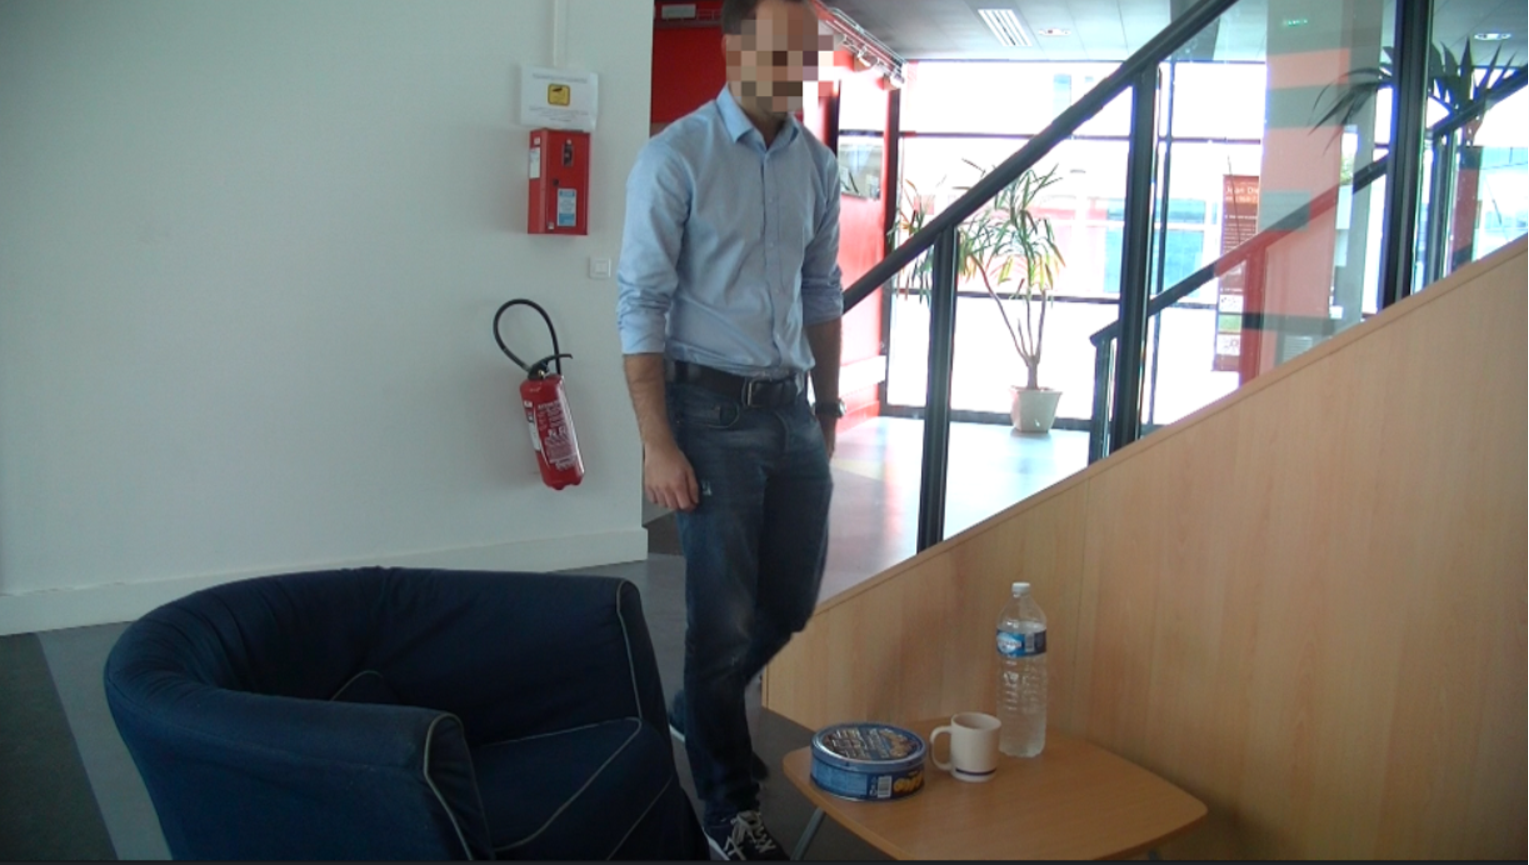
\includegraphics[scale=0.5]{img/observer/cookie1-blur.pdf}
	\caption{The cookie intention scenario}
	\label{fig:observer_experiments-cookie}
\end{figure}


\subsection{Keys Scenario}
\begin{itemize}
\item Objects: a \textit{Box} was placed on the \textit{Table}, that partially occluded the sight of people approaching. A \textit{Book} and a \textit{Mug} where placed behind the \textit{Box}, so that they could be seen from the sofa but not from approaching people.
\item Intentions: \textit{Taking the Mug}, \textit{Taking the Keys}, \textit{Reading the Book}.
\item Tests and Events:
\begin{itemize}
\item \textit{No Clues}: \textit{Max} approaches the \textit{Table}.
\item\textit{Contextual Clues}: \textit{Max} approaches the \textit{Table} in a hurry, while putting on a coat.
\item \textit{Divergent Belief Max}: \textit{Max} approaches the \textit{Table} in a hurry, while putting on a coat.
\end{itemize}
\item \textit{Divergent Belief Event}: \textit{Max} is sitting on the \textit{Table}, drinking from the \textit{Mug}, while having the \textit{Keys} in his hands. His phone rings, so he drops the \textit{Keys} and the \textit{Mug} on the \textit{Table}, behind the \textit{Box}, and leaves the room. While \textit{Max} is away, \textit{Bob} comes and sits on the \textit{Sofa}, reading a \textit{Book}. When he sees the \textit{Keys}, he takes them, places the \textit{Book} on the \textit{Table}, and leaves.
\end{itemize}

The \textit{Divergent Belief Event} was shown to the users (and its simulation streamed to the system) between \textit{Contextual Clues} and the \textit{Divegent Belief Max} events. This scenario can be seen in figure~\ref{fig:observer_experiments-keys}.

 \begin{figure}[ht!]
	\centering
	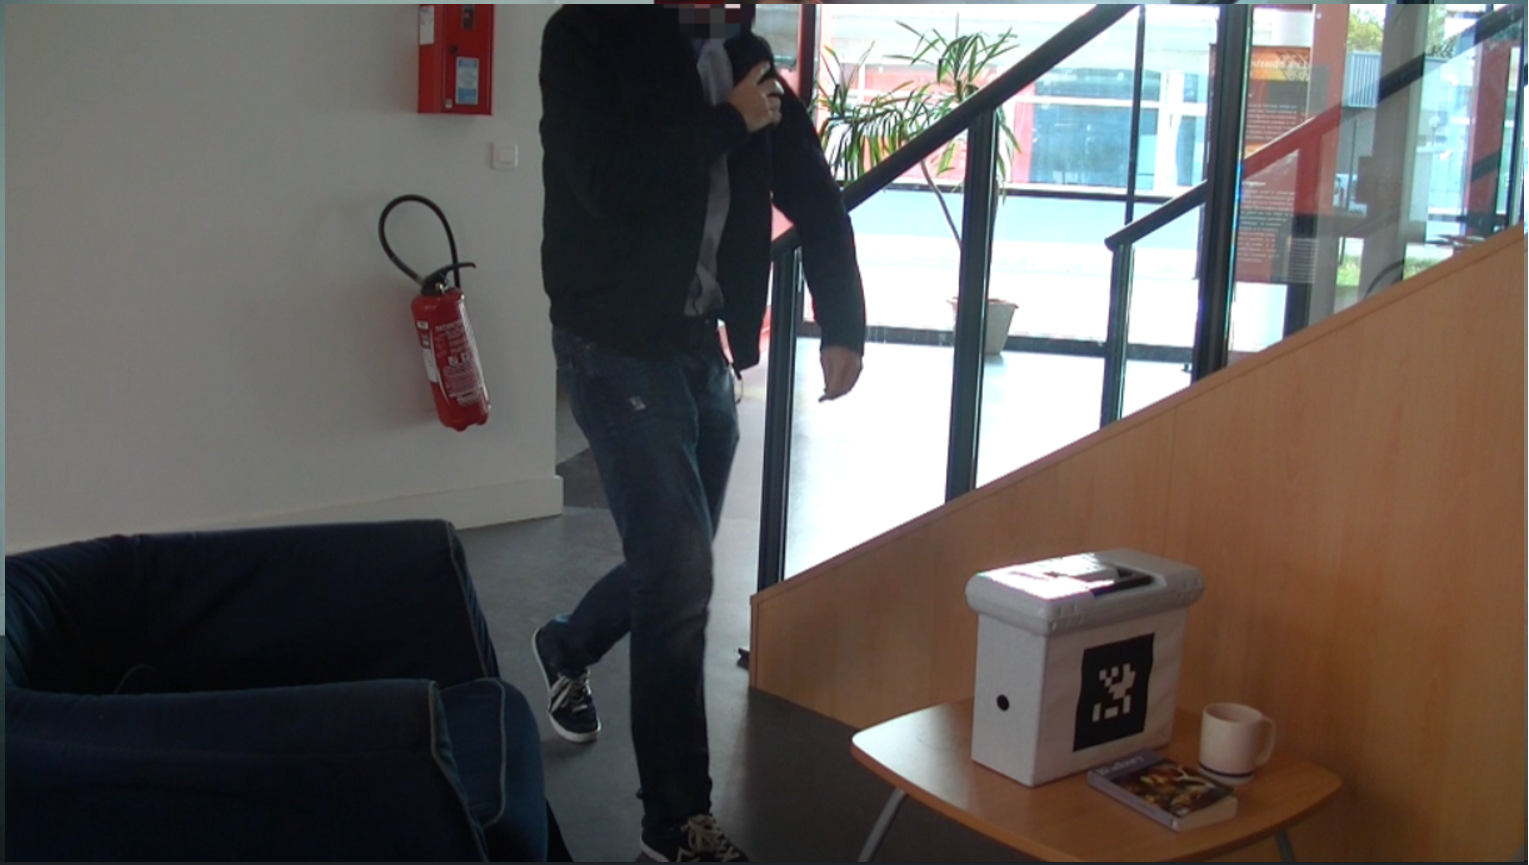
\includegraphics[scale=0.5]{img/observer/keys2-blur.pdf}
	\caption{The keys intention scenario}
	\label{fig:observer_experiments-keys}
\end{figure}

\section{Experiment}
\label{sec:observer_experiment-experiment}
\subsection{User Study}
We built an online user study, where we presented videos related to the tests and events of the two scenarios to users, who had to evaluate the likelihood of each intention of the scenario
on a five-level Likert scale. The user study was conducted in three languages, with users living in two different countries\footnote{A version of this user study was provided at http://goo.gl/forms/YiuFHnF63c}. We collected answers from 78 adults, performed an average, and converted them to percentile scores, in order to compare them with the system's predictions.

Looking at users' answers (figure \ref{fig:observer_experiments-user_study_results}), we can see that, in the absence of clues, people rated similarly the two intentions related to visible objects. Contextual clues had the highest influence on users' ratings. This is particularly visible in the \textit{Contextual Clues} test of the \textit{Keys Scenario}, where users chose as the most likely intention \textit{Take Keys}, even if no keys were visible in the video. Divergent beliefs also influenced users decisions, but not as strongly as context. The strongest responses, over all, where given by the \textit{Divergent Belief Max} test on \textit{Keys Scenario}, which uses both divergent belief and contextual information.

\subsection{System Implementation}
\label{subsec:observer_results-system_implementation}
In this subsection, we show how we implemented this experiment on our system. We will start by showing how we created a simulation of the scenarios. Then we will explain how we computed conditional dependencies between intentions and contexts, and finally we will discuss about the actual implementation of the IGs in the two scenarios.

\subsubsection{Setting up the Simulation}
% At the start of a scenario the robot scanned the environment, building a model of its world state. 
We built a simulation to represent these two scenarios. For each scenario, we set the positions of the objects and computed a starting world state.

 At the start of the scenario, the system does not have information about what each human knows, and so it will assume that they have the same belief model as itself. The system will be able to form a different belief model of each human only with the \textit{Divergent Belief} event. This is a simplification. In the real world, we believe that humans have complex mechanisms to infer others' mental beliefs, based on many aspects. For example, if we would go to the home of a friend, we would probably infer that he has knowledge even about attributes that he can not immediately perceive (e.g. he will know that that he can find a glass in a cabinet in the kitchen even if he can not see it at the moment). Instead, if other people come at our home, we would infer that they do not know where objects are located until they see them. Our system is not able to replicate this idea, leading to our simplification.

 For each test of our simulation, we streamed coordinates related to the body and hand positions of agents, following what was shown in the videos of the user study. For example, if in a test we showed Max moving from the hallway to the table, we streamed a trajectory of coordinates representing this path. 

The inference process was performed by building different IGs for the scenarios. Each test had a different graph, related to its main agent. 

\subsubsection{Contextual Information}
We considered three different Context Nodes for our simulation: \textit{Hot Day}, true when the day is particularly warm; \textit{Break Time}, true when the agents are taking a pause; \textit{Time to Leave}, true when it is late in the day, and the humans usually leave work and return home.

As previously said, we have chosen to follow \cite{Liu2014} in order to learn the link between Context and Intention Nodes. We submitted a questionnaire to 15 users with 16 questions, representing every possible combination of the intentions and contexts used in our scenarios. In each question,
the users had to rate how they perceived that a context influenced a particular intention. The rating was based on a five-level Likert scale, representing the range (\textit{very negatively}, \textit{very positively}). For example, one of the questions asked how a very warm day would influence the probability that the user would drink water.

The conditional dependency between intention $I_i$ and context $C_j$ was computed in the following way: 
\begin{equation}
 P(I_i|C_j=1)=\frac{\sum_{k=1}^5 ncj_k \times v_k}{n\_users}
\end{equation}

where $ncj_k$ is the number of persons who rated the influence of context $C_j$ on intention $I_i$ with the value $k$, $v_k$ is the probability value that we associated to $k$ (where 1=0.1, 2=0.3, 3=0.5, 4=0.7, 5=0.9) and $n\_users=15$ is the number of users that participated in the test.

We set the values of Context Nodes manually in the tests, depending  on the information shown in the videos. While we simulated this aspect, we will give some ideas on how the values of these Context Nodes could be inferred in a real scenario.

\begin{itemize}
\item \textit{Hot Day}. The temperature of the day could be measured by a sensor or obtained from a meteo application. Also, in one of the tests Max is commenting that the day is very warm. A speech recognition software could capture this information.
\item \textit{Break Time} and \textit{Time to Leave}. These information could be either hardcoded (e.g. in the company, workers have an hour of break from 13 to 14 and leave at 17:30) or learnt by observing the agents' activities.
\end{itemize}



\subsubsection{Cookie Scenario}
The starting world state for the cookie scenario is shown in table~\ref{table:observer_results-system_starting_state_cookie}.

 \begin{table}[h!]
\centering
\scriptsize
\renewcommand{\arraystretch}{1.3}
\begin{tabular}{|c|c|}
\hline
MUG isAt TABLE    \\ \hline
BOTTLE isAt TABLE  \\ \hline
COOKIEBOX isAt TABLE   \\ \hline
COOKIEBOX capacity 1    \\ \hline
COOKIES\_SUPPLY isAt KITCHEN    \\ \hline
\end{tabular}
\caption[Starting World State for the Cookie Scenario]{The starting world state for the cookie scenario.}
 \label{table:observer_results-system_starting_state_cookie}    
\end{table}


 With our perception capacities, we would not be able to detect if the cookie box is full or empty, and so we consider it as full (using the attribute $capacity$, which can have a value of 1 or 0) at the start of a test, and update its value using the $postconditions$ of inferred human actions. We consider the box as empty when we infer that a human has taken a cookie from inside, and as full when we infer that a human has put a cookie in it.


In the \textit{Cookie Scenario} the graph for the tests is constructed from the following nodes:
\begin{itemize}
\item Context Nodes: \textit{Hot Day}, \textit{Break Time}, \textit{Time to Leave}
\item Intention Nodes: \textit{Fill Cookie Box}, \textit{Eat Cookie}, \textit{Drink Water}, \textit{Read Book}.
\item Action Nodes: \textit{Move to Table}, \textit{Move to Kitchen}.
\item Observation Nodes: distance of the agent's body and hand to each action's associated \textit{target}.
\end{itemize}

We introduce the \textit{Fill Cookie Box} intention, not present in the human test, to allow the system to detect when Bob fills the \textit{Cookie Box} during the \textit{Divergent Belief Event}.

As previously said, we set Context Nodes to plausible values, that could be extracted by watching the videos. For the \textit{Contextual Clues} test, we set the value of \textit{Hot Day} to true (since Max is commenting about the temperature), and \textit{Break Time} and \textit{Time to Leave} to false (since no data in the video points to one of these contexts being true. Max and Bob seem to have taken a break from work before the other events are shown, in the Divergent Belief Event).

\textit{Divergent Belief Event}, \textit{Divergent Belief No Cookie}, and \textit{Divergent Belief Cookie} were streamed sequentially to the system, which updated the agents' mental models and created new IGs accordingly.
After the \textit{Divergent Belief Event}, the robot inferred that Max has a divergent belief on the \textit{Cookie Box}, because he does not know that Bob filled it. The mental states of the two humans, at this point, is shown in table~\ref{table:observer_results-divergent_event}.


\begin{table}[h!]
\centering
\scriptsize
\renewcommand{\arraystretch}{1.3}
\begin{tabular}{|c|c|}
\hline
Bob & Max \\ \hline \hline
MUG isAt TABLE   & MUG isAt TABLE \\ \hline
BOTTLE isAt TABLE  & BOTTLE isAt TABLE \\ \hline
COOKIEBOX isAt TABLE   & COOKIEBOX isAt TABLE \\ \hline
COOKIEBOX capacity 1  & COOKIEBOX capacity 0   \\ \hline
COOKIES\_SUPPLY isAt KITCHEN & COOKIEBOX\_SUPPLY isAt KITCHEN  \\ \hline
\end{tabular}
\caption[Belief models of Max And Bob after the Divergent Belief Event]{The table shows the belief models of Max and Bob after the Divergent Belief Event. } 
 \label{table:observer_results-divergent_event}    
\end{table}



 During the \textit{Divergent Belief Event} several IGs need to be created with different Action and Observation Nodes, to follow the sequence of actions by the two agents. For example, when \textit{Max} leaves the room, \textit{Bob} has the possibility to execute the actions \textit{Take Mug}, \textit{Take Water Bottle}, \textit{Open Cookie Box}, \textit{Move to Kitchen Shelf} or \textit{Leave Room}. Intention and Context nodes remains the same in all the IGs of the scenario.



\subsubsection{Keys Scenario}
The starting world state for the keys scenario is shown in table~\ref{table:observer_results-system_starting_state_keys}.

 \begin{table}[h!]
\centering
\scriptsize
\renewcommand{\arraystretch}{1.3}
\begin{tabular}{|c|c|}
\hline
BOX isAt TABLE    \\ \hline
BOOK isAt TABLE  \\ \hline
MUG isAt TABLE   \\ \hline
\end{tabular}
\caption[Starting World State for the Keys Scenario]{The starting world state for the keys scenario.}
 \label{table:observer_results-system_starting_state_keys}    
\end{table}

The IG for this scenario is similar to the one for the \textit{Cookie Scenario}, with the following differences.
\begin{itemize}
\item Context Nodes: \textit{Hot Day}, \textit{Break Time} and \textit{Time to Leave}.
\item Intention Nodes: \textit{Drink Water}, \textit{Take Keys}, \textit{Read Book}.
\end{itemize}

Action Nodes and Observation Nodes are the same as the previous scenario, and follow the same ideas during the \textit{Divergent Belief Event}. An example of IG used in the tests can be seen in figure \ref{fig:intention-intention_graph}, presented in chapter~\ref{chapter:intention}. For the \textit{Contextual Clues} and \textit{Divergent Belief} test, we set the \textit{Time to Leave} context value to \textit{true} (since Max is putting on a coat and seems in a hurry), and other Context Node values to \textit{false}. Using the component described in the chapter~\ref{chapter:intention} and these IGs the system was able to obtain predictions from the user actions.

\section{Discussion}
\label{sec:observer_experiment-discussion}
We performed TOST tests for each intention in the scenarios, comparing the humans' answers with the system's, for a total of 21 tests. We calculated p-values and performed our tests using a significance value $\alpha=0.05$.

Analyzing the results of our equivalence tests, shown in figure \ref{fig:observer_experiments-user_study_results}, produces some interesting information.
\begin{itemize}
\item \textbf{The behavior of our system is often close to human capacities}. 16 tests out of 21 passed our requirements   with very low p-value scores. 
\item \textbf{Context and Divergent Belief are necessary}. A system without these skills would only have been able to model properly the \textit{No Clues} cases. 
\item \textbf{There are still some missing aspects in our system}. 
	\begin{itemize}
		\item When our system does not find a strategy to achieve a goal, the probability of the related intention is inferred as zero. Humans, instead, perform a different kind of reasoning. This is particularly evident in the \textit{Contextual Clues} test of the \textit{Keys Scenario}, where our system produced very different results than the users' answers. In this case, contextual information made users think that Max wanted to take the keys, even if no keys where actually present. Somehow, humans are able to infer the mental belief of Max, deducing that maybe he thinks that there are keys on the table. Our system is not able to replicate this reasoning.
		\item In some situations it seems that humans perform complex temporal reasonings. In the \textit{Divergent Belief Cookie} of the \textit{Cookie Scenario}, the users' average answer for the \textit{Eat Cookie} intention was quite high. We believe that users thought that, since Bob, in the previous videos, filled the box, probably he wants to eat a cookie. Contextual information about the warmth of the day where less strong in this case. 
	\end{itemize}

\end{itemize}
 \begin{figure}[ht!]
	\centering
	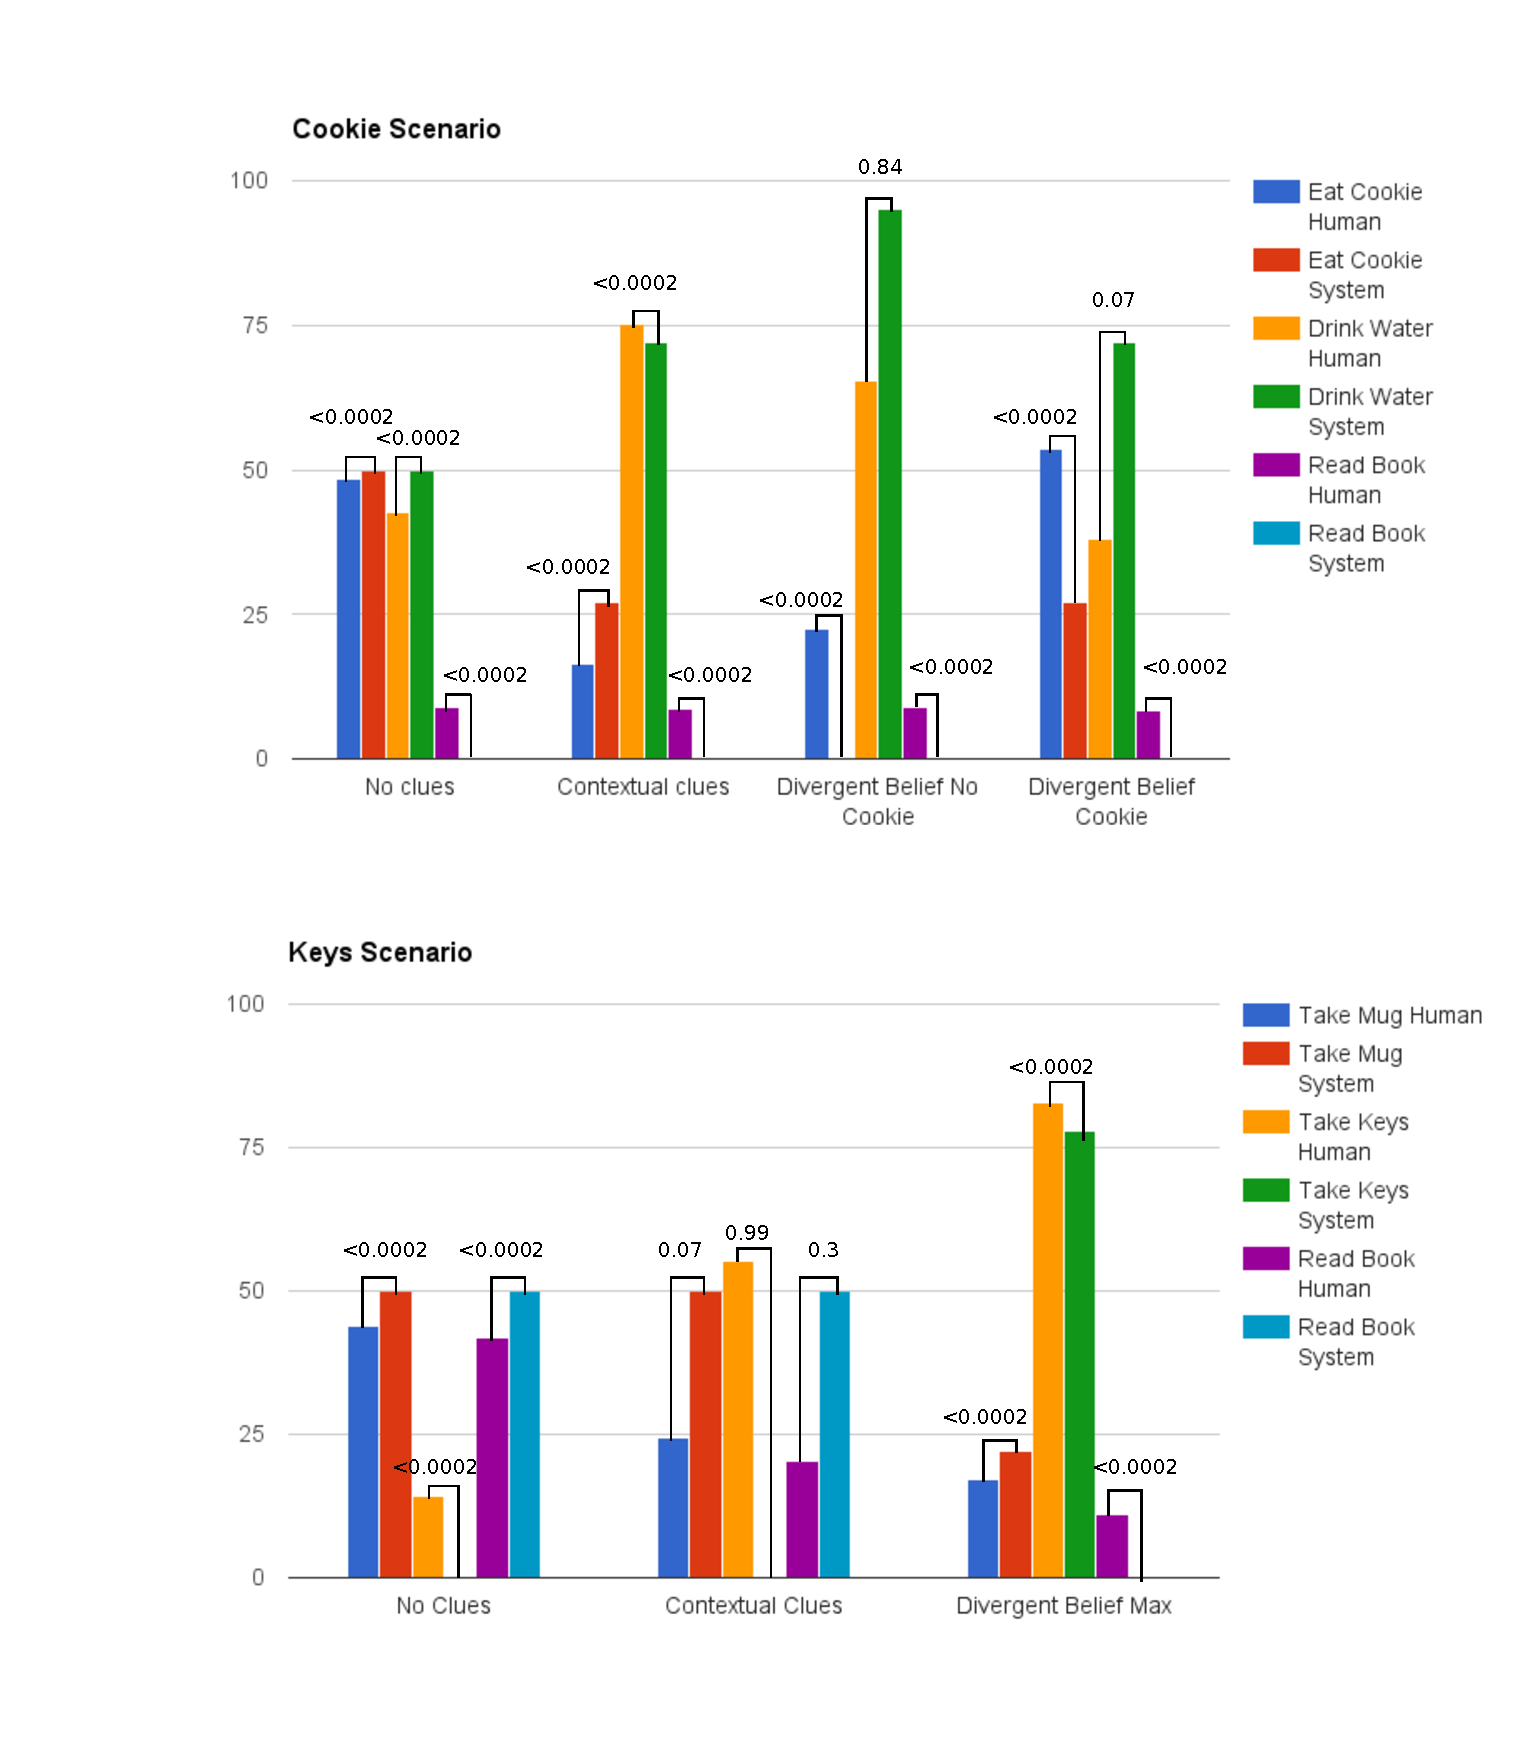
\includegraphics[clip,scale=0.7]{img/observer/scenarios_redone_1.pdf}
	\caption[Experiment results]{Experiment results. Results from the two scenarios are represented as graphs. Intentions, as estimated by the humans and the system, are represented by different colors, as shown in the legend of the graphs, with estimations of the same intention by the system or the human placed in adjacent positions. Each column represents the likelihood of an intention, expressed as a percentile score. P-values from the equivalence tests are shown, linking the estimation of an intention by the humans and by the system.}
	\label{fig:observer_experiments-user_study_results}
\end{figure}



